\chapter{Batch Normalization}
In this chapter, we discuss the batch normalization (BN) technique. The aim of BN is to avoid gradient explosion or disappearance, which makes the training process unstable, i.e. the gradient is either too large or too small to be a reasonable update.

\section{The Definition of Batch Normalization}
BN can be applied to any layer of a neural network, where it normalizes, scales and shifts an internal computation result. It in fact includes two parts, one for the training procedure and one for the test.

\subsection{Model w.r.t loss function: an idea to ``understand" BN}
In fact, BN is just a new model, and then use the general SGD w.r.t mini-batch type! The new model of BN is like:
\begin{equation}\label{BN-model}
L(\Theta) = \sum_{i \in I} \frac{1}{|N|} \|\tilde {f}^J(x_i;\Theta) - y_i\|^2,
\end{equation}
as $I = \{1, 2,\cdots,N\}$ is the {\bf all data}.  
We can rewrite it as:
\begin{equation}\label{BN-model1}
L(\Theta) = \mathbb{E}_{i} \|\tilde {f}^J(x_i;\Theta) - y_i\|^2.
\end{equation}
Now we define $\tilde {f}^J(x_i;\Theta)$ as:
\begin{equation}
\tilde f^j = \theta^j \circ \text{\text{BN}}_{I} ( g^j\circ\tilde f^{j-1}).
\end{equation}
or, as it may perform better in practice,
\begin{equation}
\tilde f^j = \theta^j \circ g^j \circ \text{\text{BN}}_{I} (\tilde f^{j-1}),
\end{equation}
So what we will explain is based the second form.
At layer $j$, with a scaling factor $\gamma^j\in\mathbb{R}$ and a shifting $\beta^j \in \mathbb{R}$, $\text{BN}_I$ is defined as
\begin{equation}
\text{BN}_{I}(x)= \gamma^j\frac{x - \mu_I^j}{\sigma_I^j}+\beta^j \bm{1},
\end{equation}
where $\mu^j$ is the mean value and $\sigma^j$ is the standard deviation of the all date i.e.
\begin{align}
\mu_I^j &= \frac{\sum_{i\in I}  x_i }{|I|},\\
\sigma_I^j  &= \sqrt{ \delta + \frac{ \sum_{i\in I} ( x_i - \mu_I^j)^2}{|I|-1} }.
\end{align}
where $\delta$ is an extra term for numerical stability, and the square in $(  x_i - \mu^j)^2$ is an element-wise square operation.

Note that $\gamma^j$ and $\beta^j$ are parameters to be trained.

If BN is added after the linear transformation, i.e.
\begin{equation}
\text{BN}_I(f^{j-1}(X_i))=\text{BN}_{I}(WX_i + b),
\end{equation}
the bias $b$ is in fact removed by BN, thus
\begin{equation}
\text{BN}_I(f^{j-1}(X_i))=\text{BN}_I(WX_i).
\end{equation}


\subsection{Training Process:  approximated SGD}
Now to train BN model, we still use SGD, so we just sample a subset of data as $S \subset I$ and compute gradient on this mini-batch.  

{\bf But to compute the $\mu^j_I$ is very expensive, and we can simply use the idea in statistics i.e use the sampled data $S$ to approximate $I$.} 

So for every step, the corresponding object function to be take gradient can be written as:
\begin{equation}
	\sum_{i \in S} \|\tilde {f}^J(x_i) - y_i\|^2,
\end{equation}
where for each layer $\tilde f^j$,
\begin{equation}
\tilde f^j = \theta^j \circ \text{\text{BN}}_{S} ( g^j\circ\tilde f^{j-1}).
\end{equation}
or, as it may perform better in practice,
\begin{equation}
\tilde f^j = \theta^j \circ g^j \circ \text{\text{BN}}_{S} (\tilde f^{j-1}),
\end{equation}
So what we will explain is based the second form.

At layer $j$, with a scaling factor $\gamma^j\in\mathbb{R}$ and a shifting $\beta^j \in \mathbb{R}$, $\text{BN}_S$ is defined as
\begin{equation}
\text{BN}_{S}(x)= \gamma^j\frac{x - \mu_S^j}{\sigma_S^j}+\beta^j \bm{1},
\end{equation}
where $\mu^j$ is the mean value and $\sigma^j$ is the standard deviation of the input mini-batch, i.e.
\begin{align}
\mu^j_I \approx \mu_S^j &= \frac{\sum_{i\in S}  x_i }{|S|},\\
\mu_I^j \approx \sigma_S^j  &= \sqrt{ \delta + \frac{ \sum_{i\in S} ( x_i - \mu_S^j)^2}{|S|-1} }.
\end{align}
where $\delta$ is an extra term for numerical stability, and the square in $(  x_i - \mu^j)^2$ is an element-wise square operation.

Note that $\gamma^j$ and $\beta^j$ are parameters to be trained.

With the trainable parameters in $\text{BN}_S$, the derivative now becomes
\begin{align}
\frac{\partial \tilde f^j}{ \partial \theta^{j-1}} &= \theta^j \circ (g^j)' \circ \frac{\partial \text{BN}_{S} (\tilde f^{j-1})}{ \partial \theta^{j-1}} \\
&=  \theta^j \circ (g^j)' \circ \left(\frac{\partial \text{BN}_{S} (\tilde f^{j-1})}{ \partial \mu^j}\frac{\partial \mu^j}{\partial \theta^j} + \frac{\partial \text{BN}_{S} (\tilde f^{j-1})}{ \partial \sigma^j}\frac{\partial \sigma^j}{\partial \theta^j} + \frac{\partial \text{BN}_{S} (\tilde f^{j-1})}{ \partial \tilde f^j}\frac{\partial \tilde f^j}{\partial \theta^j}  \right).
\end{align}
The gradient of $\gamma$ and $\beta$ are trivial. The back-propagation process can then be applied to optimize the model.

\subsection{Testing Process: recover $\mu_I$ and $\sigma_I$ from all samples}
Considering that a mini-batch is an approximation of the whole dataset, the mean value $\mu$ and standard deviation $\sigma$ of BN in each layer, should be the same, all being of the whole dataset.


%at the testing time, they are replaced by those of the whole dataset, i.e.
%\begin{align}\label{bnbatch}
%	\mu_I&\approx \mu = \frac{1}{n_\mathcal{B}}\sum_{B\in\mathcal{B}}\mu_B,\\
%	\sigma^2_I&\approx \sigma^2 = \frac{1}{n_\mathcal{B}}\sum_{B\in\mathcal{B}}\sigma^2_{\mathcal{B}},
%\end{align}
%where $\mathcal{B}$ is the set of all mini-batches.
Thus, after optimizing the model,  use the moving average scheme as:
\begin{equation}\label{BN-timeaverage}
\mu_t=\rho*\mu_t+(1-\rho)*\bar\mu_{t-1} \quad \sigma_t=\rho*\beta_t+(1-\rho)*\bar\sigma_{t-1},
\end{equation}
with $\mu_t$ and $\sigma_t$ is the $\mu_{S_t}$ and $\sigma_{S_t}$ in step t. {\bf But we don't use the updated $\mu_{S_t}$ or $\sigma_{S_t}$ in training phase, we just note them and use for approximate the real $\mu_I$ and $\sigma_I$ in previous BN model.} 

The parameters $\gamma$ and $\beta$ will be kept.

\subsection{Implementation of batch normalization}
Batch normalization (BN) can be viewed as a function $\text{BN}(x)$, where

\begin{enumerate}
	\item in 1D case, $x\in\mathbb{R}^{m\times C\times n}$,
	\item in 2D case, $x\in\mathbb{R}^{m\times C\times H \times W}$,
	\item in 3D case, $x\in \mathbb{R}^{m\times C\times D \times H \times W}$.
\end{enumerate}
What matters is $m$, the number of input samples, and $C$, the number of channels.

$H$, $W$, $D$ means height, width, and depth respectively, in 2D or 3D case, and $n$ simply means the length of a sample in 1D case.

Because only $m$ and $C$ are necessary for BN, we will denote $x_{i,c}$ as a tensor, where $i$, $c$ is the first and the second index of $x$, i.e. the dimension of $n$, $H$, $W$, $D$ are omitted.

The definition of $\text{BN}(x)$, denoted as $y$, is
\begin{equation}
	\begin{aligned}
		y&=\text{BN}(x),\\
		y_{i,c}&=\gamma_c\frac{x_{i,c}-\text{mean}_i[x_{i,c}]}{\sqrt[]{\text{Var}_i[x_{i,c}]+\epsilon}}+\beta_c,
	\end{aligned}
\end{equation}
where $\text{mean}_i[x_{i,c}]$ is the mean of $x_{i,c},\ i\in I$ and $\text{Var}_i[x_{i,c}]$ is the variance of $x_i, i\ \in I$. $\gamma_c,\beta_c\in\mathbb{R}$ are the trainable parameters, often called the scale and the shift, respectively. $\epsilon$ is used for numerical stability.

In the training process, like all the other parameters such as $W$ and $b$, $\gamma,\beta$ will be updated with $\nabla_\gamma L$ and $\nabla_\beta L$, where $L$ is the loss function. 

In practice, mean $\mu$ and var $\sigma$ are in fact the running estimates $\bar\mu$, $\bar\sigma$, i.e. 
\begin{equation}
	\begin{aligned}
		&\text{Initialize running estimates, }&\bar\mu_0=0,\ \bar\sigma_0=1,\\
		&\text{At time step t, compute mean and var, }&\mu_t=\text{mean}_i[x_{i,c}],\ \sigma_t=\text{Var}_i[x_{i,c}],\\
		&\text{Update running estimates, }&\bar\mu_t=\rho*\mu_t+(1-\rho)*\bar\mu_{t-1},\\
		&&\bar\sigma_t=\rho*\beta_t+(1-\rho)*\bar\sigma_{t-1},\\
	\end{aligned}
\end{equation}
where $\rho$ is the momentum, $\rho\in(0,1)$ and $\rho\approx 0.1$ in practice.

In the testing process, the final $\bar\mu$ and $\bar\sigma$ are used to normalize the input.

BN is often used before activation functions, e.g. a one-hidden-layer neural network with BN can be written as
\begin{equation}
	\label{bn_1hidden}
	f(x)=\theta_2\circ \text{ReLU1}\circ\text{BN}\circ\theta_1\circ x.
\end{equation}

\begin{figure}[htbp]
	\centering{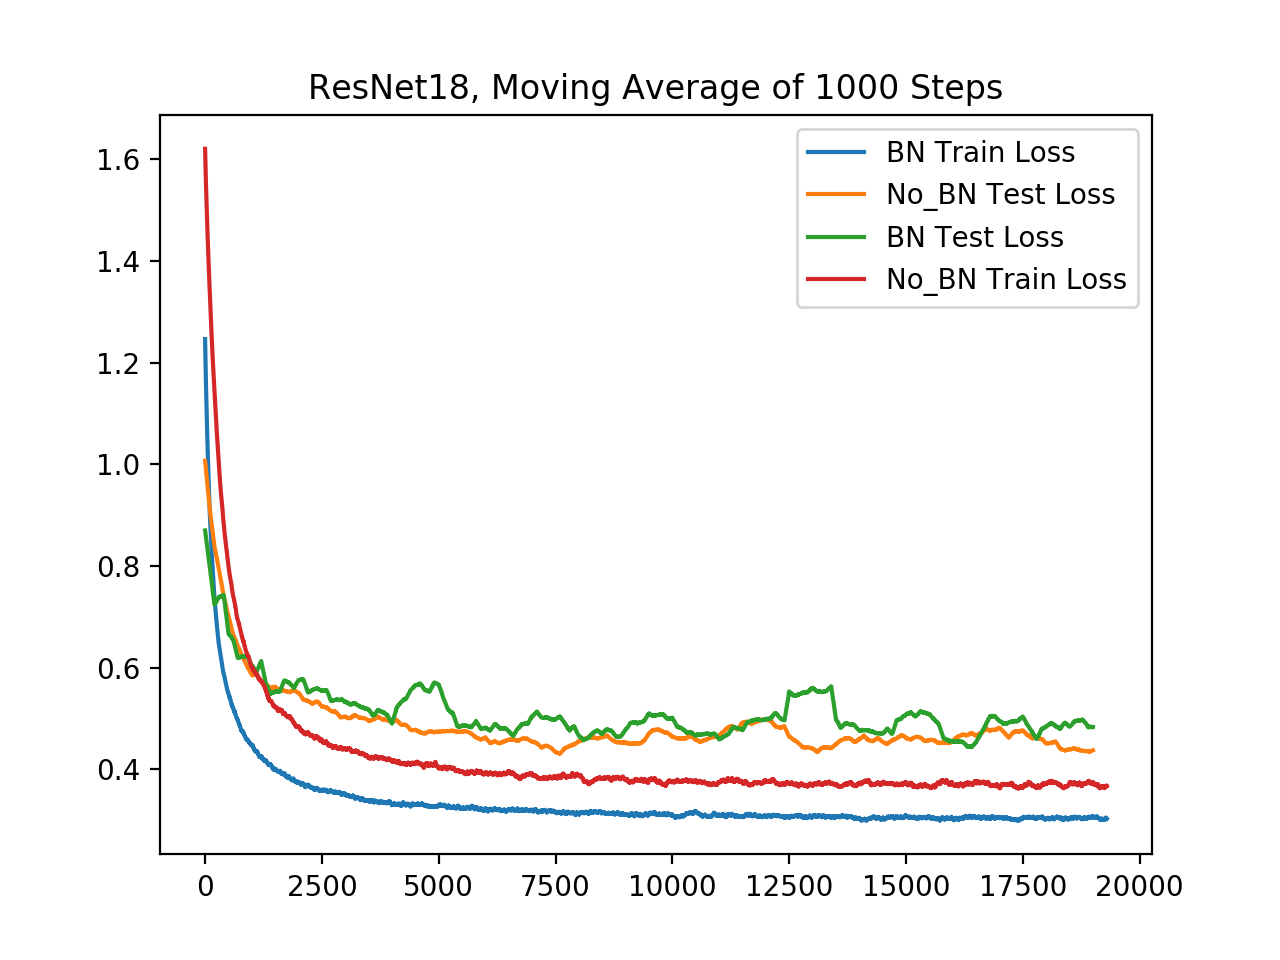
\includegraphics[width=10cm]{BN_NoBN.png}}
	\caption{Comparison of BN on ResNet10, CIFAR-10}
	\label{alo: large k}
\end{figure}

%{\bf For test phase}, to the $\hat \mu^j$ and $\hat \sigma^j$ are computed
%by averaging those $\mu^j$ and $\sigma^j$ in training phase. In training phase, suppose we have those next training process with mini-batch $S_t$ for $t = 1:T$. So, after $T$ steps gradient descent, those $\theta^j$ have been trained well, and we get:
%\begin{equation}
%\mu^j_{t}, \sigma^j_t, \quad t = 1:T,
%\end{equation}
%So the test model is
%\begin{equation}
%f(x) = \hat{f}^J(x),
%\end{equation}
%with
%\begin{equation}
% \hat{f}^j(x) = \theta^j \circ g^j \circ \hat{\text{BN}}^j(\hat f^{j-1})
%\end{equation}
%for
%\begin{equation}
%\hat{\text{BN}}^j( \hat f^{j-1}(x_i) )= \frac{\hat f^{j-1}(x_i) - \hat \mu^j}{\hat \sigma^j},
%\end{equation}
%where
%\begin{equation}
%\hat \mu^j =\frac{\sum_{i=1}^T \mu^j_t }{T},
%\end{equation}
%and
%\begin{equation}
%\hat \sigma^j  = \frac{\sum_{i=1}^T \sigma^j_t }{T}.
%\end{equation}
%
%In some situation, they may use the similar strategy like the momentum for SGD, then may get $\hat \mu^j$ and $\hat \sigma^j$ by: For $t= 1 :T$
%\begin{equation}
%\hat \mu^j = 0.9 \hat \mu^j + 0.1 \mu^j_t,
%\end{equation}
%and the similar operation for $\hat \sigma^j$

\subsection{An example}
Now consider a simple case in the Deep Learning Book, where
\begin{enumerate}
\item there's no activation function,
\item all layers have only one neuron and no bias, i.e. $\theta(x) = wx$.
\end{enumerate}
$f$ is further defined to have $J$ layers, i.e.
\begin{equation}
	f(x) = w_J w_{J-1} \cdots w_2 w_1 x,
\end{equation}
with the loss function
\begin{equation}
	L(w_1, \cdots, w_J) = \sum_{i = 1}^N\frac{1}{2} (f(x_i) - y_i)^2.
\end{equation}
The gradients can then be computed as
\begin{align}
	\frac{\partial L}{\partial f(x_i)}&=f(x_i)-y_i,\\
	\frac{\partial f}{\partial w_i}&=\frac{f(x)}{w_i}=x\prod_{j\neq i}w_j.
\end{align}
The problem is that, if $w_j,2\leq j\leq J$ are updated with $\epsilon\Delta w_j$, the update of $w_1$ would be 
\begin{equation}
	\frac{\partial f}{\partial w_1}=x\prod_{j\geq2}(w_j+\epsilon\Delta w_j),
\end{equation}
which multiplies the change of parameters, and when $J$ is larger, the effect is stronger. If the change is scaling up, this may introduce gradient explosion, or disappearance if it's scaling down.

One may adjust the learning rate $\epsilon$ to moderate this effect, but this is hard in practice.

%Now we suppose to decrease the value for $f$ by $0.1$ at $x$. With the first order approximation of $f$, we know that $f$ will decrease about
%\begin{equation}
%\epsilon \|\bm{g}\|^2,
%\end{equation}
%with
%\begin{equation}
%\bm{w} \leftarrow \bm{w} - \epsilon \bm{g}.
%\end{equation}
%
%However, for really situation, we have
%\begin{equation}
%f(x) = (w_J - \epsilon g_J)\cdots(w_1 - \epsilon g_1)x.
%\end{equation}
%For one term in seconder approximation like:
%\begin{equation}
%\epsilon^2 g_1 g_2 \Pi_{i=3}^J w_i x.
%\end{equation}
%Because we connot control the value of $\Pi_{i=3}^J w_i x$, it can be very small or extremely large so {\bf it it very difficult to choose suitable learning rate.}

With BN, the model is changed to
\begin{equation}
\tilde f(x) = w_J \tilde f^{J-1}(x),
\end{equation}
where the update is normalized.
%with $\tilde f^{J-1}$ has the stander statistics( or $\gamma$ and $\eta$ by adaptivity). If we don't use \text{BN}, we know that for any $w_j$ with $j = 1:J-1$ can effect the $f(x)$ remarkably like $w_j = 0$ makes this network degeneration or $w_j = -w_j$ changes the prediction of $f(x)$ totally. Without normalization, nearly every update would have an extreme effect on the statistics of $f^{J-1}$.
%
%Now suppose that $x$ is drawn from a unit Gaussian i.e:
%\begin{equation}
%x \sim \mathcal{N}(0,1).
%\end{equation}
% Then the original method $f$ is also Gaussian but not unit it depended w.r.t $\bm{w}$:
%\begin{equation}
%f \sim \mathcal{N}(\mu({\bm{w}}),\sigma(\bm{w})).
%\end{equation}
%But if we use \text{BN}, here $\tilde h^{J-1}$ becomes unit Gaussian again, i.e
%\begin{equation}
%\tilde f^{J-1} \sim \mathcal{N}(0,1).
%\end{equation}  So $\tilde f$ is an Gaussian only depends on $\omega_J$,
%\begin{equation}
%\tilde f \sim \mathcal{N}(\mu(w_J),\sigma(w_J)).
%\end{equation}  which means we just need to trained $w_J$ all $w_j$ for $j=1:J-1$ make no sense for this model. So, what we only need to train is only $w_J$, this make the training process very fast.

As it says in the book,
\begin{quotation}
	\emph{
		Batch normalization has thus made this model significantly easier to learn. In this example, the ease of learning of course came at the cost of making the lower layers useless. In our linear example, the lower layers no longer have any harmful effect, but they also no longer have any beneficial effect. This is because we have normalized out the first and second order statistics, which is all that a linear network can influence. In a deep neural network with nonlinear activation functions, the lower layers can perform nonlinear transformations of the data, so they remain useful. Batch normalization acts to standardize only the mean and variance of each unit in order to stabilize learning, but allows the relationships between units and the nonlinear statistics of a single unit to change.}
\end{quotation}

%\section{XN: A normalization method based on ReLU1}
This section introduces a new kind of parameters normalization methods based on Prof. Xu's idea for ReLU1 activation function.

\subsection{XN in progress}
Suppose we have a dataset $\mathcal{X}\subset\mathbb{R}^n$, which has $N$ samples, each sample $x\in \mathcal{X}$ with a label $y_x=e_i,i=1,2,...,c$, where $c$ is the number of classes.

Consider a one-hidden-layer neural network 
\begin{equation}
	\label{1hidden}
	f(x)=W_2\text{ReLU1}(W_1x+b_1)+b_2,  
\end{equation}
where $W_1\in\mathbb{R}^{n_1\times n},\ W_2\in\mathbb{R}^{c\times n_1}$, and a loss function \[L(X)=\frac{1}{N}\sum_{x\in X}\|f(x)-y_x\|^2_2,\] where $x\in\mathbb{R}^n$ is a sample and $y_x=e_i$ is the label. 
%\subsubsection{Version 1}
%\begin{enumerate}
%	\item For an full-batch input matrix $X\in\mathbb{R}^{n\times N}$, where each column of $X$ is a sample, find the rows $y$ of $W_1X+b_1$ s.t. the $i$th element of $y$, denoted as $y_i$, satisfying
%	\begin{equation}
%		y_i\notin [0,1], \quad\forall i.
%	\end{equation}
%	Denoted the corresponding rows of $W_1$ and $b_1$ as $\bar W$ and $\bar b$.
%	\item Solve the optimization problem
%	\begin{equation}
%		\begin{aligned}
%			\min_{W,b}&\quad\|WX+b - \text{ReLU1}(\bar WX+\bar b)\|_F\\
%			\text{subject to}&\quad (WX+b)_{ij}\leq 0\text{ or } \geq 1,\quad \forall i,j.
%		\end{aligned}
%	\end{equation}
%
%	\item Replace $\bar W$ and $\bar b$ by $W$ and $b$.
%\end{enumerate}
\subsubsection{XN Version 2}
XN is independent with the SGD training process.

After an update of the neural network, XN can be applied to each hidden layer successively, and won't change the output of it. In this example, we have only one hidden layer. The XN algorithm can be written as follows.
\begin{enumerate}
	\item Denote $\Theta=(W_1\ b_1)\in\mathbb{R}^{n_1\times(n+1)}$, $\hat X=(X;\mathbf{1})\in\mathbb{R}^{(n+1)\times m}$ and $Y=\text{ReLU1}(W_1X+b_1)$. 
	Split the columns of $\hat X$ to $X_I$, $X_J$, $X_K$, s.t. for every row $\theta_i$ of $\Theta$, $i=1,...,n_1$,
	\begin{equation}
	\begin{aligned}
	\theta_i X_I\leq 0,\\
	\theta_i X_J\geq 1,\\
	\theta_i X_K\in[0,1].
	\end{aligned}
	\end{equation}
	Denote IJ as the union of I and J. For every $\theta_i$, the optimization problem can be rewritten as
	\begin{equation}\label{standardv2opt}
	\begin{aligned}
	\min_\theta&\quad\|\theta  X_{IJ}-Y_{IJ}\|_2\\
	\text{subject to}&\quad\theta X_{I}\leq 0,\\
	&\quad\theta X_{J}\geq 1,\\
	&\quad\theta X_{K}=Y_{K}.
	\end{aligned}
	\end{equation}
	
	\paragraph{Note}
	\begin{enumerate}
	\item
	If $X_K$ is row full-rank, the problem has only one solution, which is the original $w_1,b_1$.
	\begin{proof}
		Because $X_K$ is row full-rank, we have, by definition,
		\begin{equation}
		xX_K=0\Rightarrow x=0.
		\end{equation}
		If there are $\theta$, $\theta'$ s.t.
		\begin{equation}
		\theta X_K=Y_K,\quad \theta' X_K=Y_K,
		\end{equation}
		then
		\begin{equation}
		(\theta-\theta') X_K=0\Rightarrow \theta-\theta'=0.
		\end{equation}
	\end{proof}
	\item
	In practice, the cases when the equality constraint 
	\begin{equation}
		\theta X_K=Y_K
	\end{equation}
    is under-determined	appear after several epochs of SGD training.
	\item
	\ref{standardv2opt} is a standard constraint optimization problem, with inequality constraints. It has no explicit solution, and can be solved by algorithms such as interior-point methods, the simplex algorithm, etc. In practice, we may turn to standard libraries to solve it.

	\end{enumerate}
%	\begin{equation}\label{v2opt}
%		\begin{aligned}
%			\min_{W,b}&\quad\|(WX+b - \text{ReLU1}(W_1X+b_1)\|_F\\
%			\text{subject to}&\quad (WX+b)_{ij}<0\text{ or } >1,\quad \forall (i,j)\in Z,\\
%			&\quad (WX+b)_{ij}=(W_1X+b_1)_{ij},\quad \forall (i,j)\notin Z.
%		\end{aligned}
%	\end{equation}
%
%	\eqref{v2opt} is equivalent to solve 
%	\begin{equation}\label{v2eq}
%		WX-b=Y,\quad Y_{ij}=(W_1X+b_1)_{ij},\quad \forall (i,j)\notin Z,
%	\end{equation}
%	which is in some sense easier to solve when $Z$ is larger. If $N<n+1$, \eqref{v2eq} is undetermined in most cases, however this is hard to satisfy.
	\item Replace $W_1$ and $b_1$ by $W$ and $b$. 
\end{enumerate}

%Consider \eqref{v2opt}. Denote $\Theta=(W\ b)\in\mathbb{R}^{n_1\times(n+1)}$, $\hat X=(X;\mathbf{1})\in\mathbb{R}^{(n+1)\times m}$ and $Y=\text{ReLU1}(W_1X+b_1)$, 
%\begin{equation}\label{simplifiedv2opt}
%	\begin{aligned}
%		\min_\Theta&\quad\|\Theta \hat X-Y\|_F\\
%		\text{subject to}&\quad(\Theta\hat X)_{ij}>1\ or\ <0,\quad \forall(i,j)\in Z,\\
%		&\quad(\Theta\hat X)_{ij}=Y_{ij},\quad \forall (i,j)\notin Z.
%	\end{aligned}
%\end{equation}


\subsubsection{Numerical experiments}
Our network has two hidden layers, and XN will be applied to the first, second and both hidden layers, separately, i.e. after each update, which is SGD,
\begin{enumerate}
	\item apply XN to the first hidden-layer, or
	\item apply XN to the first and the second hidden-layer, or
	\item apply XN to the second hidden-layer.
\end{enumerate}
\begin{enumerate}
%	\item \textbf{Version 1.} In \eqref{v1}, no row $y$ of $W_1X+b_1$ satisfies $y_i\notin[0,1],\forall i$, no matter which layer to apply XN. In fact, there are always almost a half of $y_i\in[0,1]$.
	\item \textbf{XN Version 2.} 
	
	Whether XN is used or not depends on the equality constraints and the error.
	
	Figure \ref{XNv2_Points} shows the loss function on point-separation problem, with XN on different layers. XN is applied only at a few time steps, as follows,
	\begin{enumerate}
		\item L, XN. 
		
		[0, 1, 2, 3, 4, 5, 6, 7, 8, 12, 14, 15, 16, 17, 34, 35, 36, 101, 102, 975, 978, 982, 987, 988, 989, 1126, 1127, 1128, 1134, 1136, 1141, 1144, 1158, 1163, 1168, 1170, 1171, 1172, 1173, 11411, 11910, 11920, 11922, 11923, 17831, 17836, 17864, 17901, 17902, 17914, 17916].
		\item XN, XN. Only second layer uses XN. 
		
		[0, 1, 2, 3, 4, 5, 6, 7, 8, 9, 10, 11, 12, 14, 17, 18, 115, 127, 16179, 16229, 16240, 16243, 16244, 16248, 16250].
		
		\item XN, L. No layer uses XN.
	\end{enumerate}
	
	\begin{figure}[H]
		\center
		\includegraphics*[width=0.8\textwidth]{./figures/XNv2_Points.png}
		\caption{Loss function on point-separation problem. [2, 20, 64, 9] shows the number of neurons at each layer (one input, two hidden, and one output layer). ['L', 'XN'] means hidden-layer 1 is Linear, and hidden-layer 2 applies XN.}
		\label{XNv2_Points}
	\end{figure}
%	In \eqref{standardv2opt}, if $\theta X_{K}=Y_{K}$ is overdetermined (for MNIST, it's may be overdetermined, because $X_K\in\mathbb{R}^{129\times m'}$, $m'\approx 30000$ (the size of the full-batch is 60000)), and 
	\begin{figure}[H]
		\center
		\includegraphics*[width=0.8\textwidth]{./figures/XNv2_mnist100.png}
		\caption{Loss function on 100 samples of MNIST. \emph{blank} means without XN.}
		\label{XNv2_Points}
	\end{figure}
	
	\begin{figure}[H]
		\center
		\includegraphics*[width=0.8\textwidth]{./figures/XNv2_mnist500.png}
		\caption{Loss function on 500 samples of MNIST. \emph{blank} means without XN. XN is applied successfully after every epoch.}
		\label{XNv2_Points}
	\end{figure}

	\begin{figure}[H]
		\center
		\includegraphics*[width=0.8\textwidth]{./figures/XNv2_mnist500_XN0.png}
		\caption{Loss function on 500 samples of MNIST. XN is applied once before SGD.}
		\label{XNv2_Points}
	\end{figure}
	
\end{enumerate}

\subsubsection{Problems}
\begin{enumerate}
	\item 
	The optimization problem is very large and the main matrix, $X_{IJ}X_{IJ}^T$, is not SPD, which means the solution is not unique. These make the solving process very time-consuming. This may be worked around by not requiring an optimal solution, but only a slightly better one.
	\item
	XN ia not directly applicable for the full MNIST dataset, because the equality constraint is over-determined at each epoch.
	\item
	The generalization ability of XN on MNIST is hard to test, because the subset dataset is too small, and, as a result, both SGD with XN and blank SGD can not make good prediction with it.
\end{enumerate}


\subsection{An example of XN (mini-batch version)}
Suppose we have a dataset $\mathcal{X}\subset\mathbb{R}^n$, which has $N$ samples, each sample $x\in \mathcal{X}$ with a label $y_x=e_i,i=1,2,...,c$, where $c$ is the number of classes.

Consider a one-hidden-layer neural network 
\begin{equation}
  \label{1hidden}
f(x)=W_2\text{ReLU1}(W_1x+b_1)+b_2,  
\end{equation}
where $W_1\in\mathbb{R}^{n_1\times n},\ W_2\in\mathbb{R}^{c\times n_1}$, and a loss function \[L(X)=\frac{1}{N}\sum_{x\in X}\|f(x)-y_x\|^2_2,\] where $x\in\mathbb{R}^n$ is a sample and $y_x=e_i$ is the label.

To train $f$ with XN, we have the following algorithm.
\begin{enumerate}
	\item Choose an $m$-sample mini-batch $X\subset\mathcal{X}$ randomly. $X$ is represented as a matrix $X\in\mathbb{R}^{n\times m}$ , where each column of $X$ is a sample.
	\item Compute the value $f_1$ of the hidden layer on $X$,
	\begin{equation}
		f_1(X)=
		\begin{pmatrix}
			W_1 & b_1
		\end{pmatrix}
		\begin{pmatrix}
			X \\ \mathbf{1}
		\end{pmatrix}
		\in\mathbb{R}^{n_1\times m}
	\end{equation}
	and the value $f_2$ of the output layer,
	\begin{equation}
		f_2(x)=
		\begin{pmatrix}
		W_2 & b_2
		\end{pmatrix}
		\begin{pmatrix}
		\text{ReLU1}(f_1(X)) \\ \mathbf{1}
		\end{pmatrix}
		\in\mathbb{R}^{c\times m}.
	\end{equation}
	\item (XN) Change the parameters of the hidden layer $W_1$, $b_1$ to $W$, $b$ such that
	\begin{equation}
		\begin{pmatrix}
			W & b
		\end{pmatrix}
		\begin{pmatrix}
			X \\ \mathbf{1}
		\end{pmatrix}
		=
		\text{ReLU1}\left(
		\begin{pmatrix}
			W_1 & b_1
		\end{pmatrix}
		\begin{pmatrix}
			X \\ \mathbf{1}
		\end{pmatrix}\right)
		=\text{ReLU1}(f_1(X)).
	\end{equation}
	Denote $\Theta=(W\ b)\in\mathbb{R}^{n_1\times(n+1)}$, $\hat X=(X;\mathbf{1})\in\mathbb{R}^{(n+1)\times m}$ and $Y=\text{ReLU1}(f_1(X))\in\mathbb{R}^{n_1\times m}$, the above equation can be rewritten as 
	\begin{equation}\label{XNeq}
		\Theta \hat X=Y.
	\end{equation} 
	The least square problem 
	\begin{equation}\label{XNlst}
		\min_\Theta\|\Theta \hat X-Y\|_F
	\end{equation}
	gives a solution of \eqref{XNeq} if the minimal value is $0$. To assure $0$ is reachable, note that \eqref{XNeq} can be expanded as
	\begin{equation}
		\bar X\bar\Theta=\bar Y,\quad
		\bar X\in\mathbb{R}^{n_1m\times(nn_1+n_1)},\ \bar\Theta\in\mathbb{R}^{nn_1+n_1},\ \bar Y\in\mathbb{R}^{n_1m\times(nn_1+n_1)},
	\end{equation}
	so we can make $\bar X$ an underdetermined matrix by requiring $n_1m < nn_1+n_1$, or
	\begin{equation}
		m < n+1.
	\end{equation}
	That is to say, in a layer, the number of input samples should not be larger than the dimension of a sample. \eqref{XNlst} can then be solved by LAPACK package directly. 
	If \eqref{XNlst} is not solvable, for example because of a $\bar X$ with a zero-row, then XN is not applied, i.e. $W_1,\ b_1$ is not changed.
	
	\textbf{Notes}. 
	\begin{enumerate}
		\item Because $\hat X$ is not necessarily square, a plausible way to solve \eqref{XNeq} is by pseudo-inverse,
		\begin{align*}
		\Theta \hat X=Y&\Rightarrow\Theta \hat X{\hat X}^T=Y{\hat X}^T\\
		&\Leftrightarrow\Theta =Y{\hat X}^T(\hat X{\hat X}^T)^{-1}.
		\end{align*}
		However, because $\hat X\in\mathbb{R}^{(n+1)\times m}$ and we require $m<n+1$, $\hat X{\hat X}^T$ is not invertible. Even if $\hat X{\hat X}^T$ is invertible, we can not get $\Theta \hat X=Y$ if $\hat X$ is not invertible. If it is, we can solve the equation directly with $\hat X^{-1}$.
		\item Another way is to assume $\Theta=Z\bar X^T$, and we have
		\begin{align*}\\
		\Theta \hat X=Y&\Leftrightarrow Z\bar X^T \hat X=Y\\
		&\Leftrightarrow Z =Y({\hat X}^T\hat X)^{-1}.\\
		&\Rightarrow
		\Theta=Y({\hat X}^T\hat X)^{-1}\bar{X}^T.
		\end{align*}
		This is a feasible method. However, this method won't bring an obviously difference as the least square method, so we won't show the results of it.
	\end{enumerate}
	
	\item Update the parameters with gradient descent methods on the mini-batch.
	\item Go to 1 until a convergence.
\end{enumerate}

For a fully connected neural network with several hidden layers, we just change parameters at each layer successively. The above example shows the XN algorithm on mini-batches.
\subsection{XN and ReLU1}
ReLU1, denoted as $\tau$, is defined as 
\begin{equation}
\tau(x) =
	\begin{cases}
		0 \quad & 0 < x, \\
		x \quad &0 \le x < 1, \\
		1 \quad &1 \le  x.
	\end{cases}
\end{equation}

This function has two inflection points $x=0$ and $x=1$. When $x\leq0$ or $x\geq1$, the gradient of $\tau$ is 
\begin{equation}
	\frac{\D\tau}{\D x}=0.
\end{equation}

In the above example, for an input $\mathbf{x}=\Theta\hat X$, $\tau$ is applied to each element, thus does not change the dimension of $\mathbf{x}$.

The idea of XN is to adjust $\Theta$ so that if $\mathbf{x}_{ij}\notin [0,1]$, $\mathbf{x}_{ij}$ is moved to the nearest inflection point, as shown in \eqref{XNeq}. XN does not affect the output of each layer, thus does not change the model.

Recall that a neural network is defined as $f^J$, where
\begin{equation}
f^j = \theta^j \circ g^j \circ f^{j-1},\quad j=1,2,...,J.
\end{equation}

%With XN, the function is rewritten as
%
%\begin{equation}
%	f^j = \theta^j \circ \text{ReLU1} \circ\text{XN}\circ f^{j-1},\quad j=1,2,...,J.
%\end{equation}
%Note that
%\begin{equation}\label{key}
%	\text{XN}\circ f^{j-1}=\text{XN}\circ \theta^j \circ g^{j-1},
%\end{equation}
%the operator XN in fact changes $\theta^{j-1}$ to $\theta^*$, where
%\begin{equation}
%	\theta^*\circ g^{j-1}=\text{ReLU1}\circ f^{j-1}.
%\end{equation}
%
%Denote $\text{ReLU1}\circ f^{j-1}$ on a mini-batch $B$ as $G\in\mathbb{R}^{n\times m}$, where $m$ is the size of mini-batch and $n$ is the dimension of the input, and $g^{j-1}$ on $B$ as $\bar G$, we have
%\begin{equation}
%\theta\circ g^{j-1}=
%\begin{pmatrix}
%	\bar G^T & 1_m
%\end{pmatrix}
%\begin{pmatrix}
%	W^T\\b
%\end{pmatrix}
%:=\bar X\Theta=G.
%\end{equation}
%
%The above equation can then be viewed as an optimization problem
%\begin{align}\label{op_xn}
%	\min_{\Theta\in\mathbb{R}^{n_x}}\|\bar X\Theta-G\|_F,
%\end{align}
%which may have infinite solutions, in which case we may add a constraint to it, such as $\min \|\theta-\bar\theta\|$ or $\min\|\theta\|$. However, any solution of \eqref{op_xn} is adoptable.
%
%Another quick way to solve \eqref{op_xn} is as follows. Assuming $\Theta_k=\bar X^T y,k=1,2,...,n$, we have
%\begin{align*}
%	\bar X\bar X^Ty&=G_k,\\
%	y&=(\bar X\bar X^T)^{-1}G_k,\\
%	\Theta_k&=\bar{X}^T(\bar X\bar X^T)^{-1}G_k.
%\end{align*}
%
%To guarantee $(\bar X\bar X^T)^{-1}$ exists, a necessary condition is $m<n$.
%
%One can also use a package to compute the linear square problem directly. For example, in Python, numpy.linalg.lstsq() provides such an API. This function in facts uses LAPACK library, which further uses divide and conquer methods to solve the problem.
% 
%The algorithms are as follows. 

\begin{algorithm}[htb]
	\caption{Training Algorithm with XN}
	\label{alg0_XN}
	\begin{algorithmic}[1]
		\Require $\Theta_0$, learning rate $\eta_t$
		\For{$t = 0,1 \cdots$}
		\State Select a mini-bath $B_t$.
		\State Replace $\Theta_t$ with $\hat{\Theta}_t$,
		\begin{equation}
			\Theta_t\leftarrow \hat{\Theta}_t = \text{XN}(f^J, \Theta_t, B_t).
		\end{equation}
		\State Compute the gradient (BP),
		\begin{equation}
			g_t = \nabla_{\Theta} L_{B_t}(\Theta) |_{\Theta = \hat{\Theta}_t}.
		\end{equation}
		\State Update parameters $\Theta$ with
		\begin{equation}
			\Theta_{t+1} = \Theta_{t} - \eta_t g_t.
		\end{equation}
		\EndFor
	\end{algorithmic}
\end{algorithm}

\begin{algorithm}[htb]
\caption{XN: solve $\hat \Theta_t$ from $\Theta_t$ and $f^J$ on $B_t$}
\label{XN_solve}
\begin{algorithmic}[1]
\Require The neural network $f^J$,  current parameters $\Theta_t$, mini-batch $B_t$
\For{$j = 0:J-1$}
\For{$k = 1:n_{j+1}$}
\State Compute $\hat \theta^j_{t,k}$ such that
\begin{equation}\label{eq1:XN}
\hat{\theta}_{t,k}^j \bar{x}^j_i = g^{j+1}({\theta}_{t,k}^j \bar{x}^j_i),
\end{equation}
with $x^j_i = g^j(f^{j-1}(x_i))$ for $i \in B_t$. For example, $\theta=\bar{X}^T(\bar X\bar X^T)^{-1}g$.

\State Replace $\hat\theta$ by $\theta$,
\begin{equation}
	\hat\theta\leftarrow\theta.
\end{equation}
%\State If \eqref{eq1:XN} have infinite solutions, we can add those kind of constrains:
%\begin{equation}\label{eq1:constrain}
%\min \|\hat{\theta}_{t,k}^j  - \theta_{t,k}^j\|^2  \quad \text{or} \quad \min  \|\hat{\theta}_{t,k}^j  - \theta_{t,k}^j\|_{1}
%\end{equation}
\EndFor
\EndFor
\end{algorithmic}
\end{algorithm}

\section{Implementation}

XN is implemented with PyTorch as an independent layer object.

\section{Numerical Results}

We use a fully connected neural network, with two hidden layers, each has 100 neurons. Thus, the mini-batch size should be smaller than 101.

We will only do XN on the second hidden layer.

We want XN to be properly solved, so there is a parameter \emph{xn\_error} to control the error, i.e.
\begin{equation}
	\|\Theta \hat X-Y\|_F<\text{xn\_error}.
\end{equation}

A max-norm is more convenient, because it's not sensitive to batch-size. We still use F-norm here.

Also, we have two methods to solve XN, i.e. the least square and the pseudo-inverse one. We will denote them as \emph{lst} and \emph{inv} respectively.

We test XN on different datasets. 

\subsection{Points-separation problem}
\subsubsection{Introduction}
The samples of points-separation problem with $9$ classes are shown as follows.

\begin{figure}[H]
	\center
	\includegraphics*[width=0.5\textwidth]{./figures/XN_Points_show.png}
	\caption{The training data of 9-class points-separation problem.}
\end{figure}

This problem can be easily solved by plain SGD, i.e. without BN or XN, the prediction of which is as follows.

\begin{figure}[H]
	\center
	\includegraphics*[width=0.5\textwidth]{./figures/XN_Points_SGD_pred.png}
	\caption{The prediction of the neural network trained by plain SGD.}
\end{figure}

\subsubsection{Loss on mini-batches}

The setup is as follows. 

\begin{center}
	\begin{tabular}{|l|c|}
		\hline
		Batch size & 32\\
		\hline
		xn\_error & $10^{-4}$\\
		\hline
		Learning rate & $0.01$\\
		\hline
	\end{tabular}
\end{center}

Due to the size of xn\_error, not all training step will apply XN. Figure \ref{fig:XN_points_1} shows the value of loss function and whether using XN at each step.

\begin{figure}[H]
	\center
	\includegraphics*[width=10cm]{./figures/XN_Points.png}
	\caption{Above: loss function on mini-batch at each step; below: if using XN at each step, 1 if use XN, otherwise 0.}
	\label{fig:XN_points_1}
\end{figure}

\textbf{Observations on Figure \ref{fig:XN_points_1}} 
\begin{enumerate}
	\item Within the first 100 steps, XN decreases the loss function.
	\item After 1000 steps, although the loss function on the current mini-batch won't change, it will increase sharply on the next mini-batch. XN will break the prediction on other mini-batches.
\end{enumerate}

XN breaks the prediction on other mini-batches even without SGD, as Figure \ref{fig:XN_points_onlyXN} shows.
\begin{figure}[H]
	\center
	\includegraphics*[width=10cm]{./figures/XN_points_onlyXN.png}
	\caption{At each step, when using XN, SGD is not used.}
	\label{fig:XN_points_onlyXN}
\end{figure}


We may add a parameter xn\_prob to control the probability of using XN. By changing the probability of XN, we can see how the loss function will change. Figure \ref{fig:XN_points_02} shows loss function on mini-batches with xn\_prob=0.2.

\begin{figure}[H]
	\center
	\includegraphics*[width=10cm]{./figures/XN_Points_02.png}
	\caption{Loss function on mini-batch, with xn\_prob=0.2.}
	\label{fig:XN_points_02}
\end{figure}

\subsubsection{Train the full-batch and adjust on mini-batch}
Another way to use XN is doing gradient descent on the full-batch, and doing XN on the mini-batch.

With the same xn\_error=$10^{-4}$ and other setups, figure \ref{fig:XN_points_full} shows value of loss function on the whole training dataset.
\begin{figure}[H]
	\center
	\includegraphics*[width=10cm]{./figures/XN5.png}
	\caption{Loss on the full-batch.}
	\label{fig:XN_points_full}
\end{figure}
\textbf{Observations on Figure \ref{fig:XN_points_full}} 
\begin{enumerate}
	\item Within the first 100 steps, XN decreases the full loss function.
	\item After 1000 steps, it will increase sharply after XN. XN will break the prediction on other samples.
\end{enumerate}

We can decrease the XN error to $10^{-5}$, so  that only the first 100 steps will use XN. The loss is shown in figure \ref{fig:XN_points_full_100}. The first several XN speed up the training.
\begin{figure}[H]
	\center
	\includegraphics*[width=10cm]{./figures/XN1.png}
	\includegraphics*[width=10cm]{./figures/XN_Points_full_1e5.png}
	\caption{Loss on the full-batch. Only step 8, 21 and 50 use XN.}
	\label{fig:XN_points_full_100}
\end{figure}

\subsection{MNIST}
We now use the dataset MNIST. xn\_error is $10^{-6}$.

\subsubsection{Loss function with xn\_prob 0.2}
Figure \ref{fig:XN_MNIST_1} shows the loss function on mini-batches with XN-probability $0.2$.
\begin{figure}[H]
	\center
	\includegraphics*[width=8cm]{./figures/XN14.png}
	\caption{Loss function on mini-batches with xn\_prob $0.2$.}
	\label{fig:XN_MNIST_1}
\end{figure}

\subsubsection{Train the full-batch and adjust on mini-batch}
Using GD on the full-batch and XN on the mini-batch, Figure \ref{fig:XN_MNIST_full} shows the loss on the full training dataset.
\begin{figure}[H]
	\center
	\includegraphics*[width=8cm]{./figures/XN15.png}
	\caption{Loss function on the full-batch with xn\_prob $0.2$.}
	\label{fig:XN_MNIST_full}
\end{figure}
Decrease xn\_prob to $0.001$, we have Figure \ref{fig:XN_MNIST_full_0001} showing the loss function on the full-batch.
\begin{figure}[H]
	\center
	\includegraphics*[width=\textwidth]{./figures/XN17.png}
	\caption{Loss function on the full-batch with xn\_prob $0.001$.}
	\label{fig:XN_MNIST_full_0001}
\end{figure}

\textbf{Observations on Figure \ref{fig:XN_MNIST_full_0001}}. Every XN will increase the loss on other samples.

\subsection{Conclusion}
From the above results, although XN keeps the loss on the current mini-batch, it will increase on other samples.

Changing batch size (e.g. 2, 8, 32, 64) or learning rate (e.g. 0.1, 0.01) won't give different results, so we omit them.

To keep the loss on the full-batch is hard. First, changing $\Theta$ for a mini-batch will change the whole neural network, which will change the loss on other samples. Second, it's hard to do XN on the full-batch, because the number of the input samples, $m$, should not be larger than the dimension of a sample, $n$. $m$ is $50,000$ for MNIST full-batch, which is too large. 

\subsection{Batch Normalization}

The model VGG11 is used to compare the performance of XN, XN as loss, BN and a blank setup. ImageNet, which has $1000$ classes, is used as dataset.

VGG11 can be defined as a function $f=f_2\circ f_1$, where $f_1$ is of convolutional layers and $f_2$ is of fully connected layers,
\begin{equation}
f_2=W_3\text{ReLU1}(W_2\text{ReLU1}(W_1x+b_1)+b_2)+b_3.
\end{equation}

Dropout is used after each ReLU1 in $f_2$.

\begin{center}
	\includegraphics*[width=\textwidth]{./figures/BN_ImageNet.png}
\end{center}

The figure above compares $90$ epochs of training, with or without BN. \emph{training top1} means the accuracy of prediction on a mini-batch, and \emph{training top5} means the top5 accuracy, i.e. if the largest 5 predictions of a sample include the right one, then the prediction is viewed as correct.

\subsection{XN, XN as loss and BN, ImageNet}
\begin{center}
	\includegraphics*[width=\textwidth]{./figures/XN_ImageNet.png}
\end{center}

There are two hidden layers in $f_2$, but we only do XN on the first one. If do both, the solution of the least square problem has large error. The figure above compares the first $4000$ steps of training.

The batch size is $256$ on training data, and the optimizer is SGD with momentum $0.9$.

During the training, the error of the least square problem is kept under $10^{-4}$, except for larger numbers like $0.1$ for several times.


%\newpage
\section{Jinchao: XN}
XN is independent with the SGD training process.

After an update of the neural network, XN can be applied to each hidden layer successively, and won't change the output of it. In this example, we have only one hidden layer. The XN algorithm can be written as follows.
\begin{enumerate}
\item Denote 
$$\Theta=(W_1\ b_1)\in\mathbb{R}^{n_1\times(n+1)}$$
and
$$
\hat X=(X;\mathbf{1})\in\mathbb{R}^{(n+1)\times m}, 
Y=\text{ReLU1}(W_1X+b_1).
$$
	Split the columns of $\hat X$ to $X_I$, $X_J$, $X_K$, s.t. for every row $\theta_i$ of $\Theta$, $i=1,...,n_1$,
	\begin{equation}
	\begin{aligned}
	\theta_i X_I\leq 0,\\
	\theta_i X_J\geq 1,\\
	\theta_i X_K\in[0,1].
	\end{aligned}
	\end{equation}
	Denote IJ as the union of I and J. For every $\theta_i$, the optimization problem can be rewritten as
	\begin{equation}\label{standardv2opt}
	\begin{aligned}
	\min_\theta&\quad\|\theta  X_{IJ}-Y_{IJ}\|_2\\
	\text{subject to}&\quad\theta X_{I}\leq 0,\\
	&\quad\theta X_{J}\geq 1,\\
	&\quad\theta X_{K}=Y_{K}.
	\end{aligned}
	\end{equation}
\end{enumerate}

